
% Default to the notebook output style

    


% Inherit from the specified cell style.




    
\documentclass[11pt]{article}

    
    
    \usepackage[T1]{fontenc}
    % Nicer default font than Computer Modern for most use cases
    \usepackage{palatino}

    % Basic figure setup, for now with no caption control since it's done
    % automatically by Pandoc (which extracts ![](path) syntax from Markdown).
    \usepackage{graphicx}
    % We will generate all images so they have a width \maxwidth. This means
    % that they will get their normal width if they fit onto the page, but
    % are scaled down if they would overflow the margins.
    \makeatletter
    \def\maxwidth{\ifdim\Gin@nat@width>\linewidth\linewidth
    \else\Gin@nat@width\fi}
    \makeatother
    \let\Oldincludegraphics\includegraphics
    % Set max figure width to be 80% of text width, for now hardcoded.
    \renewcommand{\includegraphics}[1]{\Oldincludegraphics[width=.8\maxwidth]{#1}}
    % Ensure that by default, figures have no caption (until we provide a
    % proper Figure object with a Caption API and a way to capture that
    % in the conversion process - todo).
    \usepackage{caption}
    \DeclareCaptionLabelFormat{nolabel}{}
    \captionsetup{labelformat=nolabel}

    \usepackage{adjustbox} % Used to constrain images to a maximum size 
    \usepackage{xcolor} % Allow colors to be defined
    \usepackage{enumerate} % Needed for markdown enumerations to work
    \usepackage{geometry} % Used to adjust the document margins
    \usepackage{amsmath} % Equations
    \usepackage{amssymb} % Equations
    \usepackage{textcomp} % defines textquotesingle
    % Hack from http://tex.stackexchange.com/a/47451/13684:
    \AtBeginDocument{%
        \def\PYZsq{\textquotesingle}% Upright quotes in Pygmentized code
    }
    \usepackage{upquote} % Upright quotes for verbatim code
    \usepackage{eurosym} % defines \euro
    \usepackage[mathletters]{ucs} % Extended unicode (utf-8) support
    \usepackage[utf8x]{inputenc} % Allow utf-8 characters in the tex document
    \usepackage{fancyvrb} % verbatim replacement that allows latex
    \usepackage{grffile} % extends the file name processing of package graphics 
                         % to support a larger range 
    % The hyperref package gives us a pdf with properly built
    % internal navigation ('pdf bookmarks' for the table of contents,
    % internal cross-reference links, web links for URLs, etc.)
    \usepackage{hyperref}
    \usepackage{longtable} % longtable support required by pandoc >1.10
    \usepackage{booktabs}  % table support for pandoc > 1.12.2
    \usepackage[normalem]{ulem} % ulem is needed to support strikethroughs (\sout)
                                % normalem makes italics be italics, not underlines
    

    
    
    % Colors for the hyperref package
    \definecolor{urlcolor}{rgb}{0,.145,.698}
    \definecolor{linkcolor}{rgb}{.71,0.21,0.01}
    \definecolor{citecolor}{rgb}{.12,.54,.11}

    % ANSI colors
    \definecolor{ansi-black}{HTML}{3E424D}
    \definecolor{ansi-black-intense}{HTML}{282C36}
    \definecolor{ansi-red}{HTML}{E75C58}
    \definecolor{ansi-red-intense}{HTML}{B22B31}
    \definecolor{ansi-green}{HTML}{00A250}
    \definecolor{ansi-green-intense}{HTML}{007427}
    \definecolor{ansi-yellow}{HTML}{DDB62B}
    \definecolor{ansi-yellow-intense}{HTML}{B27D12}
    \definecolor{ansi-blue}{HTML}{208FFB}
    \definecolor{ansi-blue-intense}{HTML}{0065CA}
    \definecolor{ansi-magenta}{HTML}{D160C4}
    \definecolor{ansi-magenta-intense}{HTML}{A03196}
    \definecolor{ansi-cyan}{HTML}{60C6C8}
    \definecolor{ansi-cyan-intense}{HTML}{258F8F}
    \definecolor{ansi-white}{HTML}{C5C1B4}
    \definecolor{ansi-white-intense}{HTML}{A1A6B2}

    % commands and environments needed by pandoc snippets
    % extracted from the output of `pandoc -s`
    \providecommand{\tightlist}{%
      \setlength{\itemsep}{0pt}\setlength{\parskip}{0pt}}
    \DefineVerbatimEnvironment{Highlighting}{Verbatim}{commandchars=\\\{\}}
    % Add ',fontsize=\small' for more characters per line
    \newenvironment{Shaded}{}{}
    \newcommand{\KeywordTok}[1]{\textcolor[rgb]{0.00,0.44,0.13}{\textbf{{#1}}}}
    \newcommand{\DataTypeTok}[1]{\textcolor[rgb]{0.56,0.13,0.00}{{#1}}}
    \newcommand{\DecValTok}[1]{\textcolor[rgb]{0.25,0.63,0.44}{{#1}}}
    \newcommand{\BaseNTok}[1]{\textcolor[rgb]{0.25,0.63,0.44}{{#1}}}
    \newcommand{\FloatTok}[1]{\textcolor[rgb]{0.25,0.63,0.44}{{#1}}}
    \newcommand{\CharTok}[1]{\textcolor[rgb]{0.25,0.44,0.63}{{#1}}}
    \newcommand{\StringTok}[1]{\textcolor[rgb]{0.25,0.44,0.63}{{#1}}}
    \newcommand{\CommentTok}[1]{\textcolor[rgb]{0.38,0.63,0.69}{\textit{{#1}}}}
    \newcommand{\OtherTok}[1]{\textcolor[rgb]{0.00,0.44,0.13}{{#1}}}
    \newcommand{\AlertTok}[1]{\textcolor[rgb]{1.00,0.00,0.00}{\textbf{{#1}}}}
    \newcommand{\FunctionTok}[1]{\textcolor[rgb]{0.02,0.16,0.49}{{#1}}}
    \newcommand{\RegionMarkerTok}[1]{{#1}}
    \newcommand{\ErrorTok}[1]{\textcolor[rgb]{1.00,0.00,0.00}{\textbf{{#1}}}}
    \newcommand{\NormalTok}[1]{{#1}}
    
    % Additional commands for more recent versions of Pandoc
    \newcommand{\ConstantTok}[1]{\textcolor[rgb]{0.53,0.00,0.00}{{#1}}}
    \newcommand{\SpecialCharTok}[1]{\textcolor[rgb]{0.25,0.44,0.63}{{#1}}}
    \newcommand{\VerbatimStringTok}[1]{\textcolor[rgb]{0.25,0.44,0.63}{{#1}}}
    \newcommand{\SpecialStringTok}[1]{\textcolor[rgb]{0.73,0.40,0.53}{{#1}}}
    \newcommand{\ImportTok}[1]{{#1}}
    \newcommand{\DocumentationTok}[1]{\textcolor[rgb]{0.73,0.13,0.13}{\textit{{#1}}}}
    \newcommand{\AnnotationTok}[1]{\textcolor[rgb]{0.38,0.63,0.69}{\textbf{\textit{{#1}}}}}
    \newcommand{\CommentVarTok}[1]{\textcolor[rgb]{0.38,0.63,0.69}{\textbf{\textit{{#1}}}}}
    \newcommand{\VariableTok}[1]{\textcolor[rgb]{0.10,0.09,0.49}{{#1}}}
    \newcommand{\ControlFlowTok}[1]{\textcolor[rgb]{0.00,0.44,0.13}{\textbf{{#1}}}}
    \newcommand{\OperatorTok}[1]{\textcolor[rgb]{0.40,0.40,0.40}{{#1}}}
    \newcommand{\BuiltInTok}[1]{{#1}}
    \newcommand{\ExtensionTok}[1]{{#1}}
    \newcommand{\PreprocessorTok}[1]{\textcolor[rgb]{0.74,0.48,0.00}{{#1}}}
    \newcommand{\AttributeTok}[1]{\textcolor[rgb]{0.49,0.56,0.16}{{#1}}}
    \newcommand{\InformationTok}[1]{\textcolor[rgb]{0.38,0.63,0.69}{\textbf{\textit{{#1}}}}}
    \newcommand{\WarningTok}[1]{\textcolor[rgb]{0.38,0.63,0.69}{\textbf{\textit{{#1}}}}}
    
    
    % Define a nice break command that doesn't care if a line doesn't already
    % exist.
    \def\br{\hspace*{\fill} \\* }
    % Math Jax compatability definitions
    \def\gt{>}
    \def\lt{<}
    % Document parameters
    \title{Traffic sign classifier writeup}
    
    
    

    % Pygments definitions
    
\makeatletter
\def\PY@reset{\let\PY@it=\relax \let\PY@bf=\relax%
    \let\PY@ul=\relax \let\PY@tc=\relax%
    \let\PY@bc=\relax \let\PY@ff=\relax}
\def\PY@tok#1{\csname PY@tok@#1\endcsname}
\def\PY@toks#1+{\ifx\relax#1\empty\else%
    \PY@tok{#1}\expandafter\PY@toks\fi}
\def\PY@do#1{\PY@bc{\PY@tc{\PY@ul{%
    \PY@it{\PY@bf{\PY@ff{#1}}}}}}}
\def\PY#1#2{\PY@reset\PY@toks#1+\relax+\PY@do{#2}}

\expandafter\def\csname PY@tok@kt\endcsname{\def\PY@tc##1{\textcolor[rgb]{0.69,0.00,0.25}{##1}}}
\expandafter\def\csname PY@tok@kp\endcsname{\def\PY@tc##1{\textcolor[rgb]{0.00,0.50,0.00}{##1}}}
\expandafter\def\csname PY@tok@nt\endcsname{\let\PY@bf=\textbf\def\PY@tc##1{\textcolor[rgb]{0.00,0.50,0.00}{##1}}}
\expandafter\def\csname PY@tok@vg\endcsname{\def\PY@tc##1{\textcolor[rgb]{0.10,0.09,0.49}{##1}}}
\expandafter\def\csname PY@tok@il\endcsname{\def\PY@tc##1{\textcolor[rgb]{0.40,0.40,0.40}{##1}}}
\expandafter\def\csname PY@tok@o\endcsname{\def\PY@tc##1{\textcolor[rgb]{0.40,0.40,0.40}{##1}}}
\expandafter\def\csname PY@tok@cm\endcsname{\let\PY@it=\textit\def\PY@tc##1{\textcolor[rgb]{0.25,0.50,0.50}{##1}}}
\expandafter\def\csname PY@tok@nd\endcsname{\def\PY@tc##1{\textcolor[rgb]{0.67,0.13,1.00}{##1}}}
\expandafter\def\csname PY@tok@si\endcsname{\let\PY@bf=\textbf\def\PY@tc##1{\textcolor[rgb]{0.73,0.40,0.53}{##1}}}
\expandafter\def\csname PY@tok@mi\endcsname{\def\PY@tc##1{\textcolor[rgb]{0.40,0.40,0.40}{##1}}}
\expandafter\def\csname PY@tok@nv\endcsname{\def\PY@tc##1{\textcolor[rgb]{0.10,0.09,0.49}{##1}}}
\expandafter\def\csname PY@tok@gp\endcsname{\let\PY@bf=\textbf\def\PY@tc##1{\textcolor[rgb]{0.00,0.00,0.50}{##1}}}
\expandafter\def\csname PY@tok@w\endcsname{\def\PY@tc##1{\textcolor[rgb]{0.73,0.73,0.73}{##1}}}
\expandafter\def\csname PY@tok@kn\endcsname{\let\PY@bf=\textbf\def\PY@tc##1{\textcolor[rgb]{0.00,0.50,0.00}{##1}}}
\expandafter\def\csname PY@tok@bp\endcsname{\def\PY@tc##1{\textcolor[rgb]{0.00,0.50,0.00}{##1}}}
\expandafter\def\csname PY@tok@sd\endcsname{\let\PY@it=\textit\def\PY@tc##1{\textcolor[rgb]{0.73,0.13,0.13}{##1}}}
\expandafter\def\csname PY@tok@mh\endcsname{\def\PY@tc##1{\textcolor[rgb]{0.40,0.40,0.40}{##1}}}
\expandafter\def\csname PY@tok@se\endcsname{\let\PY@bf=\textbf\def\PY@tc##1{\textcolor[rgb]{0.73,0.40,0.13}{##1}}}
\expandafter\def\csname PY@tok@mb\endcsname{\def\PY@tc##1{\textcolor[rgb]{0.40,0.40,0.40}{##1}}}
\expandafter\def\csname PY@tok@c\endcsname{\let\PY@it=\textit\def\PY@tc##1{\textcolor[rgb]{0.25,0.50,0.50}{##1}}}
\expandafter\def\csname PY@tok@go\endcsname{\def\PY@tc##1{\textcolor[rgb]{0.53,0.53,0.53}{##1}}}
\expandafter\def\csname PY@tok@gi\endcsname{\def\PY@tc##1{\textcolor[rgb]{0.00,0.63,0.00}{##1}}}
\expandafter\def\csname PY@tok@ow\endcsname{\let\PY@bf=\textbf\def\PY@tc##1{\textcolor[rgb]{0.67,0.13,1.00}{##1}}}
\expandafter\def\csname PY@tok@nc\endcsname{\let\PY@bf=\textbf\def\PY@tc##1{\textcolor[rgb]{0.00,0.00,1.00}{##1}}}
\expandafter\def\csname PY@tok@nf\endcsname{\def\PY@tc##1{\textcolor[rgb]{0.00,0.00,1.00}{##1}}}
\expandafter\def\csname PY@tok@cpf\endcsname{\let\PY@it=\textit\def\PY@tc##1{\textcolor[rgb]{0.25,0.50,0.50}{##1}}}
\expandafter\def\csname PY@tok@nl\endcsname{\def\PY@tc##1{\textcolor[rgb]{0.63,0.63,0.00}{##1}}}
\expandafter\def\csname PY@tok@na\endcsname{\def\PY@tc##1{\textcolor[rgb]{0.49,0.56,0.16}{##1}}}
\expandafter\def\csname PY@tok@gt\endcsname{\def\PY@tc##1{\textcolor[rgb]{0.00,0.27,0.87}{##1}}}
\expandafter\def\csname PY@tok@gs\endcsname{\let\PY@bf=\textbf}
\expandafter\def\csname PY@tok@cp\endcsname{\def\PY@tc##1{\textcolor[rgb]{0.74,0.48,0.00}{##1}}}
\expandafter\def\csname PY@tok@cs\endcsname{\let\PY@it=\textit\def\PY@tc##1{\textcolor[rgb]{0.25,0.50,0.50}{##1}}}
\expandafter\def\csname PY@tok@vi\endcsname{\def\PY@tc##1{\textcolor[rgb]{0.10,0.09,0.49}{##1}}}
\expandafter\def\csname PY@tok@kd\endcsname{\let\PY@bf=\textbf\def\PY@tc##1{\textcolor[rgb]{0.00,0.50,0.00}{##1}}}
\expandafter\def\csname PY@tok@ni\endcsname{\let\PY@bf=\textbf\def\PY@tc##1{\textcolor[rgb]{0.60,0.60,0.60}{##1}}}
\expandafter\def\csname PY@tok@gh\endcsname{\let\PY@bf=\textbf\def\PY@tc##1{\textcolor[rgb]{0.00,0.00,0.50}{##1}}}
\expandafter\def\csname PY@tok@s2\endcsname{\def\PY@tc##1{\textcolor[rgb]{0.73,0.13,0.13}{##1}}}
\expandafter\def\csname PY@tok@s1\endcsname{\def\PY@tc##1{\textcolor[rgb]{0.73,0.13,0.13}{##1}}}
\expandafter\def\csname PY@tok@no\endcsname{\def\PY@tc##1{\textcolor[rgb]{0.53,0.00,0.00}{##1}}}
\expandafter\def\csname PY@tok@sx\endcsname{\def\PY@tc##1{\textcolor[rgb]{0.00,0.50,0.00}{##1}}}
\expandafter\def\csname PY@tok@c1\endcsname{\let\PY@it=\textit\def\PY@tc##1{\textcolor[rgb]{0.25,0.50,0.50}{##1}}}
\expandafter\def\csname PY@tok@ch\endcsname{\let\PY@it=\textit\def\PY@tc##1{\textcolor[rgb]{0.25,0.50,0.50}{##1}}}
\expandafter\def\csname PY@tok@k\endcsname{\let\PY@bf=\textbf\def\PY@tc##1{\textcolor[rgb]{0.00,0.50,0.00}{##1}}}
\expandafter\def\csname PY@tok@sb\endcsname{\def\PY@tc##1{\textcolor[rgb]{0.73,0.13,0.13}{##1}}}
\expandafter\def\csname PY@tok@vc\endcsname{\def\PY@tc##1{\textcolor[rgb]{0.10,0.09,0.49}{##1}}}
\expandafter\def\csname PY@tok@mo\endcsname{\def\PY@tc##1{\textcolor[rgb]{0.40,0.40,0.40}{##1}}}
\expandafter\def\csname PY@tok@gd\endcsname{\def\PY@tc##1{\textcolor[rgb]{0.63,0.00,0.00}{##1}}}
\expandafter\def\csname PY@tok@ss\endcsname{\def\PY@tc##1{\textcolor[rgb]{0.10,0.09,0.49}{##1}}}
\expandafter\def\csname PY@tok@nn\endcsname{\let\PY@bf=\textbf\def\PY@tc##1{\textcolor[rgb]{0.00,0.00,1.00}{##1}}}
\expandafter\def\csname PY@tok@kr\endcsname{\let\PY@bf=\textbf\def\PY@tc##1{\textcolor[rgb]{0.00,0.50,0.00}{##1}}}
\expandafter\def\csname PY@tok@ne\endcsname{\let\PY@bf=\textbf\def\PY@tc##1{\textcolor[rgb]{0.82,0.25,0.23}{##1}}}
\expandafter\def\csname PY@tok@gu\endcsname{\let\PY@bf=\textbf\def\PY@tc##1{\textcolor[rgb]{0.50,0.00,0.50}{##1}}}
\expandafter\def\csname PY@tok@sh\endcsname{\def\PY@tc##1{\textcolor[rgb]{0.73,0.13,0.13}{##1}}}
\expandafter\def\csname PY@tok@kc\endcsname{\let\PY@bf=\textbf\def\PY@tc##1{\textcolor[rgb]{0.00,0.50,0.00}{##1}}}
\expandafter\def\csname PY@tok@err\endcsname{\def\PY@bc##1{\setlength{\fboxsep}{0pt}\fcolorbox[rgb]{1.00,0.00,0.00}{1,1,1}{\strut ##1}}}
\expandafter\def\csname PY@tok@sc\endcsname{\def\PY@tc##1{\textcolor[rgb]{0.73,0.13,0.13}{##1}}}
\expandafter\def\csname PY@tok@gr\endcsname{\def\PY@tc##1{\textcolor[rgb]{1.00,0.00,0.00}{##1}}}
\expandafter\def\csname PY@tok@m\endcsname{\def\PY@tc##1{\textcolor[rgb]{0.40,0.40,0.40}{##1}}}
\expandafter\def\csname PY@tok@sr\endcsname{\def\PY@tc##1{\textcolor[rgb]{0.73,0.40,0.53}{##1}}}
\expandafter\def\csname PY@tok@ge\endcsname{\let\PY@it=\textit}
\expandafter\def\csname PY@tok@nb\endcsname{\def\PY@tc##1{\textcolor[rgb]{0.00,0.50,0.00}{##1}}}
\expandafter\def\csname PY@tok@s\endcsname{\def\PY@tc##1{\textcolor[rgb]{0.73,0.13,0.13}{##1}}}
\expandafter\def\csname PY@tok@mf\endcsname{\def\PY@tc##1{\textcolor[rgb]{0.40,0.40,0.40}{##1}}}

\def\PYZbs{\char`\\}
\def\PYZus{\char`\_}
\def\PYZob{\char`\{}
\def\PYZcb{\char`\}}
\def\PYZca{\char`\^}
\def\PYZam{\char`\&}
\def\PYZlt{\char`\<}
\def\PYZgt{\char`\>}
\def\PYZsh{\char`\#}
\def\PYZpc{\char`\%}
\def\PYZdl{\char`\$}
\def\PYZhy{\char`\-}
\def\PYZsq{\char`\'}
\def\PYZdq{\char`\"}
\def\PYZti{\char`\~}
% for compatibility with earlier versions
\def\PYZat{@}
\def\PYZlb{[}
\def\PYZrb{]}
\makeatother


    % Exact colors from NB
    \definecolor{incolor}{rgb}{0.0, 0.0, 0.5}
    \definecolor{outcolor}{rgb}{0.545, 0.0, 0.0}



    
    % Prevent overflowing lines due to hard-to-break entities
    \sloppy 
    % Setup hyperref package
    \hypersetup{
      breaklinks=true,  % so long urls are correctly broken across lines
      colorlinks=true,
      urlcolor=urlcolor,
      linkcolor=linkcolor,
      citecolor=citecolor,
      }
    % Slightly bigger margins than the latex defaults
    
    \geometry{verbose,tmargin=1in,bmargin=1in,lmargin=1in,rmargin=1in}
    
    

    \begin{document}
    
    
    \maketitle
    
    

    
    \section{\texorpdfstring{\textbf{Traffic Sign
Recognition}}{Traffic Sign Recognition}}\label{traffic-sign-recognition}

\begin{center}\rule{0.5\linewidth}{\linethickness}\end{center}

\textbf{Build a Traffic Sign Recognition Project}

The goals / steps of this project are the following: * Load the data set
(see below for links to the project data set) * Explore, summarize and
visualize the data set * Design, train and test a model architecture *
Use the model to make predictions on new images * Analyze the softmax
probabilities of the new images * Summarize the results with a written
report

\subsection{Rubric Points}\label{rubric-points}

\subsubsection{\texorpdfstring{Here I will consider the
\href{https://review.udacity.com/\#!/rubrics/481/view}{rubric points}
individually and describe how I addressed each point in my
implementation.}{Here I will consider the rubric points individually and describe how I addressed each point in my implementation.}}\label{here-i-will-consider-the-rubric-points-individually-and-describe-how-i-addressed-each-point-in-my-implementation.}

\begin{center}\rule{0.5\linewidth}{\linethickness}\end{center}

\subsubsection{Writeup / README}\label{writeup-readme}

\paragraph{1. Provide a Writeup / README that includes all the rubric
points and how you addressed each one. You can submit your writeup as
markdown or pdf. You can use this template as a guide for writing the
report. The submission includes the project
code.}\label{provide-a-writeup-readme-that-includes-all-the-rubric-points-and-how-you-addressed-each-one.-you-can-submit-your-writeup-as-markdown-or-pdf.-you-can-use-this-template-as-a-guide-for-writing-the-report.-the-submission-includes-the-project-code.}

You're reading it! also explanations are in
\href{https://github.com/adarshakb/CarND-Traffic-Sign-Classifier-Project}{project
code}

\subsubsection{Data Set Summary \&
Exploration}\label{data-set-summary-exploration}

\paragraph{1. Provide a basic summary of the data set and identify where
in your code the summary was done. In the code, the analysis should be
done using python, numpy and/or pandas methods rather than hardcoding
results
manually.}\label{provide-a-basic-summary-of-the-data-set-and-identify-where-in-your-code-the-summary-was-done.-in-the-code-the-analysis-should-be-done-using-python-numpy-andor-pandas-methods-rather-than-hardcoding-results-manually.}

The code for this step is contained in the second code cell of the
IPython notebook.

I used the pandas library to calculate summary statistics of the traffic
signs data set:

\begin{itemize}
\tightlist
\item
  Number of training examples = 39209
\item
  Number of testing examples = 12630
\item
  Image data shape = (32, 32, 3)
\item
  Number of classes = 43
\end{itemize}

\paragraph{2. Include an exploratory visualization of the dataset and
identify where the code is in your code
file.}\label{include-an-exploratory-visualization-of-the-dataset-and-identify-where-the-code-is-in-your-code-file.}

The code for this step is contained in the third code cell of the
IPython notebook.

Here is an exploratory visualization of the data set. It is a bar chart
showing how the data \ldots{}

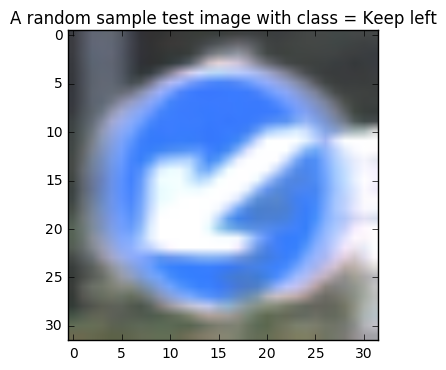
\includegraphics{./examples/example-sign.png}
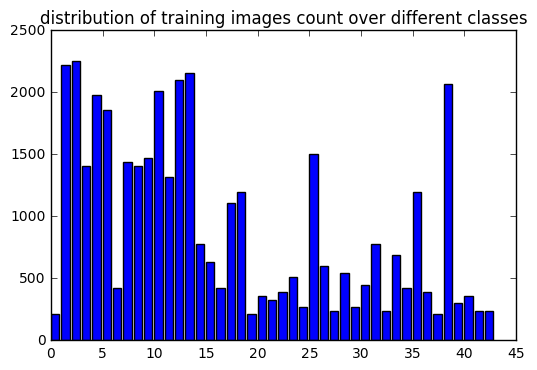
\includegraphics{./examples/visualization.png}

\subsubsection{Design and Test a Model
Architecture}\label{design-and-test-a-model-architecture}

\paragraph{1. Describe how, and identify where in your code, you
preprocessed the image data. What tecniques were chosen and why did you
choose these techniques? Consider including images showing the output of
each preprocessing technique. Pre-processing refers to techniques such
as converting to grayscale, normalization,
etc.}\label{describe-how-and-identify-where-in-your-code-you-preprocessed-the-image-data.-what-tecniques-were-chosen-and-why-did-you-choose-these-techniques-consider-including-images-showing-the-output-of-each-preprocessing-technique.-pre-processing-refers-to-techniques-such-as-converting-to-grayscale-normalization-etc.}

The code for this step is contained in the fourth code cell of the
IPython notebook.

As a first step, I decided to convert the images to grayscale because it
will reduce the number of channels and hence the number of variables
finally in the network. This means we can train better with lesser data.
However we will loose any information which might require a ``color''
component. We donot anticipate this problem here

Here is an example of a traffic sign image before and after grayscaling.

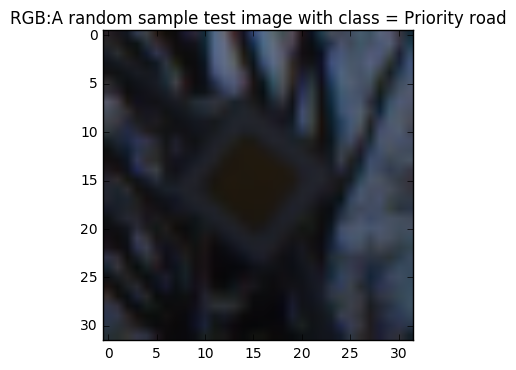
\includegraphics{./examples/grayscale-before.png}
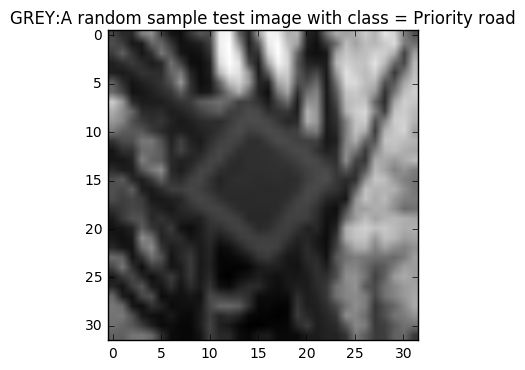
\includegraphics{./examples/grayscale-after.png}

As a last step, I normalized the image data because this will constraint
the inputs between 0 and 1 which is better for the classifier so that
there is no wide variations in the data

\paragraph{\texorpdfstring{2. Describe how, and identify where in your
code, you set up training, validation and testing data. How much data
was in each set? Explain what techniques were used to split the data
into these sets. (OPTIONAL: As described in the ``Stand Out
Suggestions'' part of the rubric, if you generated additional data for
training, describe why you decided to generate additional data, how you
generated the data, identify where in your code, and provide example
images of the additional
data)}{2. Describe how, and identify where in your code, you set up training, validation and testing data. How much data was in each set? Explain what techniques were used to split the data into these sets. (OPTIONAL: As described in the Stand Out Suggestions part of the rubric, if you generated additional data for training, describe why you decided to generate additional data, how you generated the data, identify where in your code, and provide example images of the additional data)}}\label{describe-how-and-identify-where-in-your-code-you-set-up-training-validation-and-testing-data.-how-much-data-was-in-each-set-explain-what-techniques-were-used-to-split-the-data-into-these-sets.-optional-as-described-in-the-stand-out-suggestions-part-of-the-rubric-if-you-generated-additional-data-for-training-describe-why-you-decided-to-generate-additional-data-how-you-generated-the-data-identify-where-in-your-code-and-provide-example-images-of-the-additional-data}

The code for splitting the data into training and validation sets is
contained in the fifth code cell of the IPython notebook.

To cross validate my model, I randomly split the training data into a
training set and validation set. I did this by using the buily in
train\_test\_split of sklearn which shuffles the data also.

My final training set had 31367 number of images. My validation set and
test set had 7842 and 12630 number of images.

\paragraph{3. Describe, and identify where in your code, what your final
model architecture looks like including model type, layers, layer sizes,
connectivity, etc.) Consider including a diagram and/or table describing
the final
model.}\label{describe-and-identify-where-in-your-code-what-your-final-model-architecture-looks-like-including-model-type-layers-layer-sizes-connectivity-etc.-consider-including-a-diagram-andor-table-describing-the-final-model.}

My code is based on the LeNet architecture (\textbf{with additional
modifications noted below})

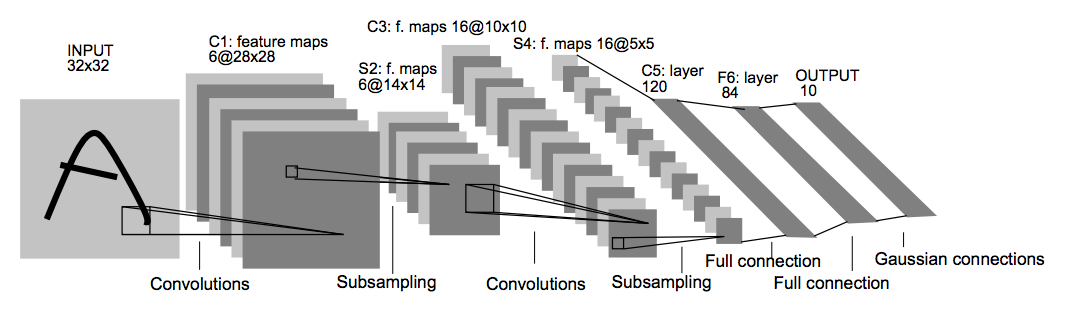
\includegraphics{./examples/lenet.png} (Image for clarity. Not the final
model)

The code for my final model is located in the 6th cell of the ipython
notebook.

My final model consisted of the following layers:

\begin{longtable}[]{@{}cc@{}}
\toprule
Layer & Description\tabularnewline
\midrule
\endhead
Input & 32x32x1 Gray scale image\tabularnewline
Convolution & 1x1 stride, same padding output 28x28x6\tabularnewline
RELU &\tabularnewline
Max pooling & 2x2 stride, outputs 14x14x6\tabularnewline
Convolution & Input 14x14x6 and output 10x10x16.\tabularnewline
RELU &\tabularnewline
Max pooling & 2x2 stride, outputs 5x5x16\tabularnewline
Flatten & convert to 1D array - 400\tabularnewline
Reduce . & 400 to 120\tabularnewline
RELU &\tabularnewline
DROPOUT & 0.5 probablity incase of training\tabularnewline
Reduce . & 120 to 84\tabularnewline
RELU &\tabularnewline
DROPOUT & 0.5 probablity incase of training\tabularnewline
Reduce . & 84 to 43 \textbf{final}\tabularnewline
Softmax & apply softmax on logits\tabularnewline
&\tabularnewline
&\tabularnewline
\bottomrule
\end{longtable}

Training with Adam Optimizer (based on gradient decent)

\paragraph{4. Describe how, and identify where in your code, you trained
your model. The discussion can include the type of optimizer, the batch
size, number of epochs and any hyperparameters such as learning
rate.}\label{describe-how-and-identify-where-in-your-code-you-trained-your-model.-the-discussion-can-include-the-type-of-optimizer-the-batch-size-number-of-epochs-and-any-hyperparameters-such-as-learning-rate.}

The code for training the model is located after the model architecture
cell of the ipython notebook.

To train the model, I used a batch size of 128 to highly parallize the
process. I also kept 100 EPOCHS as the upper limit. However I also limit
it based on validation set accuracy. I only run more EPOCHS if we are
still \emph{learning at a rate \textgreater{}= 0}. This means we donot
overfit the data w.r.t training data. The learning rate has been kept at
0.0003 so that the network is unsure at first and then becomes more
confident. I have kept the default LeNet mu \& signma hyperparameters
because I found them optimal. I also choose the mean crossentropy and
gave it to minimize for the optimizer

\paragraph{5. Describe the approach taken for finding a solution.
Include in the discussion the results on the training, validation and
test sets and where in the code these were calculated. Your approach may
have been an iterative process, in which case, outline the steps you
took to get to the final solution and why you chose those steps. Perhaps
your solution involved an already well known implementation or
architecture. In this case, discuss why you think the architecture is
suitable for the current
problem.}\label{describe-the-approach-taken-for-finding-a-solution.-include-in-the-discussion-the-results-on-the-training-validation-and-test-sets-and-where-in-the-code-these-were-calculated.-your-approach-may-have-been-an-iterative-process-in-which-case-outline-the-steps-you-took-to-get-to-the-final-solution-and-why-you-chose-those-steps.-perhaps-your-solution-involved-an-already-well-known-implementation-or-architecture.-in-this-case-discuss-why-you-think-the-architecture-is-suitable-for-the-current-problem.}

The code for calculating the accuracy of the model is located in the
16,17th cell of the Ipython notebook.

My final model results were: * validation set accuracy of 95.575\% *
test set accuracy of 89.7\%

If an iterative approach was chosen: * What was the first architecture
that was tried and why was it chosen? - I tried the architecture without
Droupout \& Also without restricting the EPOCHS if we are still
learning*.

\begin{itemize}
\tightlist
\item
  What were some problems with the initial architecture?
\item
  without dropout the results were wrong when there was a little noise
  in the images
\item
  wihtout EPOCH restriction, even tho the validation data accuracy was
  good it would overfit and get less in test data
\item
  How was the architecture adjusted and why was it adjusted? Typical
  adjustments could include choosing a different model architecture,
  adding or taking away layers (pooling, dropout, convolution, etc),
  using an activation function or changing the activation function. One
  common justification for adjusting an architecture would be due to
  over fitting or under fitting. A high accuracy on the training set but
  low accuracy on the validation set indicates over fitting; a low
  accuracy on both sets indicates under fitting.
\item
  explained above
\item
  Which parameters were tuned? How were they adjusted and why?
\item
  I tuned the learning rate. I lowered it down to get better accuracy
  prediction so that the network can start out unceratin and not overfit
\item
  What are some of the important design choices and why were they
  chosen? For example, why might a convolution layer work well with this
  problem? How might a dropout layer help with creating a successful
  model?
\item
  Dropouts help us to have redundant network connections.
\item
  ReLU help us learn complex functions in the network rather than a
  simple linear function
\item
  Maxpooling help us identify which pixel in a region is dominant ..
  such as lines or boundaries
\end{itemize}

If a well known architecture was chosen: * What architecture was chosen?
- LeNet modification * Why did you believe it would be relevant to the
traffic sign application? - LeNet has been shown to work well to
classify images * How does the final model's accuracy on the training,
validation and test set provide evidence that the model is working well?
- We have high accuracy on test set close to 90\%. These are with
certain limitations like having low number of examples in many of the
classes for the training as seen the previous barchart analysis

\subsubsection{Test a Model on New
Images}\label{test-a-model-on-new-images}

\paragraph{1. Choose five German traffic signs found on the web and
provide them in the report. For each image, discuss what quality or
qualities might be difficult to
classify.}\label{choose-five-german-traffic-signs-found-on-the-web-and-provide-them-in-the-report.-for-each-image-discuss-what-quality-or-qualities-might-be-difficult-to-classify.}

Here are five German traffic signs that I found on the web:

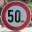
\includegraphics{./private/2-1.jpg} - might be difficult to classify due
to because it should be able to differentiate between 20/30/40/50/60 etc
signs which all look almost similar (circle \& 0 digit - about 80\% of
image are same0) 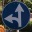
\includegraphics{./private/37-1.jpg} - might be
difficult because there is some grains in the image - its also similar
to go straight 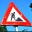
\includegraphics{./private/25-1.jpg} - the triangle is
present in many other signs 
\includegraphics{./private/18-1.jpg} -
difficult to classify as triangle is present in many other types of
signs 
\includegraphics{./private/0-1.jpg} - might be difficult to
classify due to because it should be able to differentiate between
20/30/40/50/60 etc signs which all look almost similar (circle \& 0
digit - about 80\% of image are same0)

\paragraph{\texorpdfstring{2. Discuss the model's predictions on these
new traffic signs and compare the results to predicting on the test set.
Identify where in your code predictions were made. At a minimum, discuss
what the predictions were, the accuracy on these new predictions, and
compare the accuracy to the accuracy on the test set (OPTIONAL: Discuss
the results in more detail as described in the ``Stand Out Suggestions''
part of the
rubric).}{2. Discuss the model's predictions on these new traffic signs and compare the results to predicting on the test set. Identify where in your code predictions were made. At a minimum, discuss what the predictions were, the accuracy on these new predictions, and compare the accuracy to the accuracy on the test set (OPTIONAL: Discuss the results in more detail as described in the Stand Out Suggestions part of the rubric).}}\label{discuss-the-models-predictions-on-these-new-traffic-signs-and-compare-the-results-to-predicting-on-the-test-set.-identify-where-in-your-code-predictions-were-made.-at-a-minimum-discuss-what-the-predictions-were-the-accuracy-on-these-new-predictions-and-compare-the-accuracy-to-the-accuracy-on-the-test-set-optional-discuss-the-results-in-more-detail-as-described-in-the-stand-out-suggestions-part-of-the-rubric.}

The code for making predictions on my final model is located in the
tenth cell of the Ipython notebook.

Here are the results of the prediction:

\begin{longtable}[]{@{}cc@{}}
\toprule
Image & Prediction\tabularnewline
\midrule
\endhead
Speed limit (50km/h) & Speed limit (30km/h)\tabularnewline
Go straight or left & Go straight or left\tabularnewline
Road work & Road work\tabularnewline
General caution & General caution\tabularnewline
Speed limit (20km/h) & Speed limit (30km/h)\tabularnewline
\bottomrule
\end{longtable}

The model was able to correctly guess 3 of the 5 traffic signs, which
gives an accuracy of 60\%.

\paragraph{\texorpdfstring{3. Describe how certain the model is when
predicting on each of the five new images by looking at the softmax
probabilities for each prediction and identify where in your code
softmax probabilities were outputted. Provide the top 5 softmax
probabilities for each image along with the sign type of each
probability. (OPTIONAL: as described in the ``Stand Out Suggestions''
part of the rubric, visualizations can also be provided such as bar
charts)}{3. Describe how certain the model is when predicting on each of the five new images by looking at the softmax probabilities for each prediction and identify where in your code softmax probabilities were outputted. Provide the top 5 softmax probabilities for each image along with the sign type of each probability. (OPTIONAL: as described in the Stand Out Suggestions part of the rubric, visualizations can also be provided such as bar charts)}}\label{describe-how-certain-the-model-is-when-predicting-on-each-of-the-five-new-images-by-looking-at-the-softmax-probabilities-for-each-prediction-and-identify-where-in-your-code-softmax-probabilities-were-outputted.-provide-the-top-5-softmax-probabilities-for-each-image-along-with-the-sign-type-of-each-probability.-optional-as-described-in-the-stand-out-suggestions-part-of-the-rubric-visualizations-can-also-be-provided-such-as-bar-charts}

The code for making predictions on my final model is located in the
final 2 sections of the Ipython notebook.

For the first image, the model is relatively sure that this is a stop
sign (probability of 0.6), and the image does contain a stop sign. The
top five soft max probabilities were

Image 1: - it got confused between 5 \& 3 :(
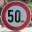
\includegraphics{./private/2-1.jpg}

\begin{longtable}[]{@{}cc@{}}
\toprule
Probability & Prediction\tabularnewline
\midrule
\endhead
.78 & Speed limit (30km/h)\tabularnewline
.20 & Speed limit (50km/h)\tabularnewline
.007 & Speed limit (80km/h)\tabularnewline
.007 & End of speed limit (80km/h)\tabularnewline
.0065 & Priority road\tabularnewline
\bottomrule
\end{longtable}

Image 2: 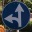
\includegraphics{./private/37-1.jpg}

\begin{longtable}[]{@{}cc@{}}
\toprule
Probability & Prediction\tabularnewline
\midrule
\endhead
.99 & Go straight or left\tabularnewline
\textasciitilde{}.00 & Keep left\tabularnewline
\textasciitilde{}.00 & Roundabout mandatory\tabularnewline
\textasciitilde{}.00 & Speed limit (70km/h)\tabularnewline
\textasciitilde{}.00 & General caution\tabularnewline
\bottomrule
\end{longtable}

Image 3: 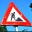
\includegraphics{./private/25-1.jpg}

\begin{longtable}[]{@{}cc@{}}
\toprule
Probability & Prediction\tabularnewline
\midrule
\endhead
.98 & Road work\tabularnewline
.01 & Bicycles crossing\tabularnewline
\textasciitilde{}.00 & Slippery road\tabularnewline
\textasciitilde{}.00 & Wild animals crossing\tabularnewline
\textasciitilde{}.00 & Beware of ice/snow\tabularnewline
\bottomrule
\end{longtable}

Image 4: 
\includegraphics{./private/18-1.jpg}

\begin{longtable}[]{@{}cc@{}}
\toprule
Probability & Prediction\tabularnewline
\midrule
\endhead
.99 & General caution\tabularnewline
.001 & Traffic signals\tabularnewline
\textasciitilde{}.00 & Pedestrians\tabularnewline
\textasciitilde{}.00 & Road narrows on the right\tabularnewline
\textasciitilde{}.00 & Bicycles crossing\tabularnewline
\bottomrule
\end{longtable}

Image 5: It got confused between 2 \& 3 :(

\includegraphics{./private/0-1.jpg}

\begin{longtable}[]{@{}cc@{}}
\toprule
Probability & Prediction\tabularnewline
\midrule
\endhead
.86 & Speed limit (30km/h)\tabularnewline
.13 & Speed limit (20km/h)\tabularnewline
.001 & Priority road\tabularnewline
\textasciitilde{}.00 & Speed limit (50km/h)\tabularnewline
\textasciitilde{}.00 & Yield\tabularnewline
\bottomrule
\end{longtable}

    \begin{Verbatim}[commandchars=\\\{\}]
{\color{incolor}In [{\color{incolor} }]:} 
\end{Verbatim}


    % Add a bibliography block to the postdoc
    
    
    
    \end{document}
